% Wei-Jin Huang -- Chinese research CV, weijincv v2
% Build from this directory:
%   latexmk -xelatex -interaction=nonstopmode -halt-on-error \
%     -jobname=wei_jin_huang_cv_weijincv_v2 cv.tex
\documentclass[10pt,a4paper]{article}

\usepackage[left=0.9cm,right=0.9cm,top=0.35cm,bottom=0.35cm]{geometry}
\usepackage{fontawesome5}
\usepackage{ctex}
\usepackage{enumitem}
\usepackage{graphicx}
\usepackage{array}
\usepackage{tabularx}
\usepackage{xcolor}
\usepackage[hidelinks]{hyperref}

\pagestyle{empty}
\setlength{\parindent}{0pt}
\setlength{\parskip}{1.5pt}
\linespread{1.08}
\sloppy

\definecolor{muted}{HTML}{4A4A4A}

% Icon, title, and full-width rule: retained from the collaborator's visual system.
\newcommand{\cvsection}[2]{%
  \vspace{5pt}%
  {\large\bfseries #1\hspace{0.5em}#2}\par
  \vspace{1pt}%
  \hrule width \linewidth height 0.6pt
  \vspace{3pt}%
}

\newcommand{\papertitle}[2]{%
  \if\relax\detokenize{#2}\relax
    \textbf{#1}%
  \else
    \href{#2}{\textbf{#1}}%
  \fi
}

% title / authors / full venue (abbreviation and year) / summary / URL
\newcommand{\paper}[5]{%
  \papertitle{#1}{#5}\par
  {\small\bfseries #3}\par
  {\color{muted}#2}\par
  \begin{itemize}[leftmargin=1.2em,topsep=2pt,itemsep=2pt,parsep=0pt,partopsep=0pt]
    \item #4
  \end{itemize}
  \vspace{3pt}%
}

% Education detail rows: equal side columns place the middle detail on the page center.
\newcommand{\edudetail}[3]{%
  \noindent
  \begin{tabularx}{\linewidth}{@{}>{\raggedright\arraybackslash}p{0.24\linewidth}@{}>{\centering\arraybackslash}X@{}>{\raggedleft\arraybackslash}p{0.24\linewidth}@{}}%
    #1 & #2 & #3
  \end{tabularx}\par
}

\begin{document}

% ============================ HEADER ========================================
\begin{center}
  \begin{minipage}[c]{0.12\linewidth}
    
\includegraphics[width=1.9cm]{figs/logo-sysu.png}
  \end{minipage}%
  \begin{minipage}[c]{0.76\linewidth}
    \centering
    {\fontsize{20}{24}\selectfont\bfseries 黄韦锦}\\[5pt]
    {\fontsize{10.5}{13}\selectfont 博士研究生\quad 计算机科学与技术\quad | \quad 中山大学\quad 广东广州}\\[5pt]
    \fontsize{10.5}{13}\selectfont
    \faEnvelope\ \href{mailto:huangwj235@mail2.sysu.edu.cn}{huangwj235@mail2.sysu.edu.cn}\hspace{2.4em}%
    \faPhone\ \href{tel:+8615089630115}{+86-15089630115}\\[5pt]
    \faGlobe\ \href{https://vkgo.github.io/}{vkgo.github.io}\hspace{2.4em}%
    \faGithub\ \href{https://github.com/vkgo}{github.com/vkgo}\hspace{2.4em}%
    \faGraduationCap\ \href{https://scholar.google.com/citations?user=jMrU_JYAAAAJ}{Google Scholar}
  \end{minipage}%
  \begin{minipage}[c]{0.12\linewidth}
    \hfill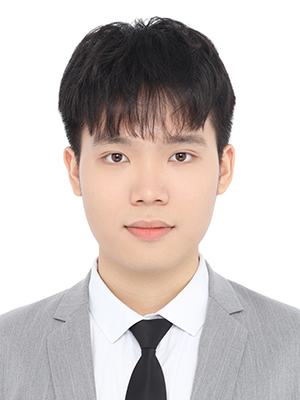
\includegraphics[width=1.9cm]{figs/photo.jpg}
  \end{minipage}
\end{center}

\vspace*{-0.45cm}

% ============================ PROFILE =======================================
\cvsection{\faUser}{研究概述}
\begin{itemize}[leftmargin=1.2em,topsep=1pt,itemsep=1pt,parsep=0pt,partopsep=0pt]
  \item \textbf{研究定位}：中山大学计算机科学与技术博士生，导师为郑伟诗教授。研究聚焦\textbf{人形机器人具身算法与视频动作理解}。
  \item \textbf{实习意向}：探索将 VLA、WAM、agentic planning 与持续学习机制相结合，利用第一视角人类数据和机器人持续交互经验，研究新任务上的组合泛化、快速适应与失败恢复。
\end{itemize}

% ============================ EDUCATION =====================================
\cvsection{\faGraduationCap}{教育经历}
\textbf{中山大学（博士）}\hfill 计算机学院—计算机科学与技术\hfill 2024.09 -- 至今\\
\edudetail{博士研究生}{研究方向：具身智能与计算机视觉}{导师：郑伟诗教授（长江学者）}

\begin{itemize}[leftmargin=1.2em,topsep=2pt,itemsep=2pt,parsep=0pt,partopsep=0pt]
  \item \textbf{荣誉奖项}：中山大学校长奖学金（前 5\%）
  \item \textbf{学术成果}：以第一/共同第一作者在 CVPR、ECCV、ACM MM 发表多篇论文。
\end{itemize}

\textbf{华南理工大学（本科）}\hfill 计算机科学与工程学院—网络工程\hfill 2020.09 -- 2024.07\\
\edudetail{工学学士}{专业排名：3/66}{}

\begin{itemize}[leftmargin=1.2em,topsep=1pt,itemsep=1pt,parsep=0pt,partopsep=0pt]
  \item \textbf{荣誉奖项}：国家奖学金（1/66）、腾讯奖学金一等奖（1/66）
  \item \textbf{竞赛获奖}：Kaggle H\&M 个性化时尚推荐竞赛银牌（85/2952，2022）、Kaggle G2Net 引力波检测竞赛银牌（57/1219，2021）
\end{itemize}

% ============================ PUBLICATIONS ==================================
\cvsection{\faBook}{代表性论文}

\paper
  {Beyond Mimicry: Learning Whole-Body Human-Humanoid Interaction from Human-Human Demonstrations}
  {\textcolor{black}{\textbf{Wei-Jin Huang}}, Yue-Yi Zhang, Yi-Lin Wei, Zhi-Wei Xia, Juantao Tan, Yuan-Ming Li, Zhilin Zhao, Wei-Shi Zheng}
  {IEEE/CVF Conference on Computer Vision and Pattern Recognition (CVPR 2026)}
  {\textbf{概述}：人形机器人全身交互缺少高质量人—机器人示范；人人交互数据更易获得，但直接重定向会因形体差异破坏关键接触，而常规模仿策略即使获得高质量数据，仍偏向轨迹复现、缺乏交互推理。PAIR 通过接触保持的物理感知重定向生成可执行的人—机器人监督；D-STAR 进一步解耦“何时动作”与“向哪里动作”的时空推理：Phase Attention 建模交互阶段，Multi-Scale Spatial 模块定位空间目标，再由 diffusion head 融合两路信息，生成同步的全身交互。}
  {https://cvpr.thecvf.com/virtual/2026/poster/37452}

\paper
  {ChoreoPlan: Hybrid Phrase Planning and Execution-Grounded Selection for Music-to-Humanoid Dance}
  {\textcolor{black}{\textbf{Wei-Jin Huang}}, Jianhong Fan, Hao Huang, Zhi-Wei Xia, Jun-Yi Deng, Yuan-Ming Li, Kun-Yu Lin, Wei-Shi Zheng}
  {ACM International Conference on Multimedia (ACM MM 2026)}
  {\textbf{概述}：音乐到人形机器人舞蹈通常先在参考动作空间规划和筛选动作，再交由全身控制器（WBC）执行；参考空间中“看起来最好”的动作，执行后未必仍然稳定、合拍，形成 reference-to-execution gap。ChoreoPlan 针对固定窗口规划难以适应音乐的变长节奏结构、参考质量无法代表执行质量这两个上游 mismatch，分别采用节拍对齐的变长离散–连续短语规划，以及基于离线 WBC rollout 的 Embodied Selector，在部署前选出兼顾可执行性与节奏/语义保持的动作。}
  {}

\paper
  {Modeling Multiple Normal Action Representations for Error Detection in Procedural Tasks}
  {\textcolor{black}{\textbf{Wei-Jin Huang}}, Yuan-Ming Li, Zhi-Wei Xia, Yu-Ming Tang, Kun-Yu Lin, Jian-Fang Hu, Wei-Shi Zheng}
  {IEEE/CVF Conference on Computer Vision and Pattern Recognition (CVPR 2025)}
  {\textbf{概述}：程序化任务错误检测中，同一执行历史后可能存在多个合法下一步；依赖固定时序或单一静态正常原型的方法会忽略这些正常未来，既难适应执行分布变化，也可能因当前动作与预测标签不一致而选错比较原型。AMNAR 根据已执行动作历史预测所有合法下一步，为每个候选动作重建自适应正常表征，再选择与当前动作最匹配的表征进行距离比较，并通过阈值判定当前动作是否异常，避免因标签预测不唯一而使用错误原型。}
  {https://openaccess.thecvf.com/content/CVPR2025/html/Huang_Modeling_Multiple_Normal_Action_Representations_for_Error_Detection_in_Procedural_CVPR_2025_paper.html}

\paper
  {EgoExo-Fitness: Towards Egocentric and Exocentric Full-Body Action Understanding}
  {Yuan-Ming Li, \textcolor{black}{\textbf{Wei-Jin Huang（共同第一作者）}}, An-Lan Wang, Ling-An Zeng, Jing-Ke Meng, Wei-Shi Zheng}
  {European Conference on Computer Vision (ECCV 2024)}
  {\textbf{概述}：第一/第三视角的全身动作理解缺少同步跨视角数据与细粒度质量标注，难以同时判断动作“做了什么、何时做、做得怎样”。EgoExo-Fitness 由 6 台相机同步采集 40 名受试者的 1,276 组跨视角序列，提供两级时序边界、动作技术要点核验、自然语言点评和质量评分，并建立动作分类、动作定位、跨视角序列验证、跨视角技能判定和指导式执行验证等基准任务，形成跨视角动作理解与可解释质量评估的完整数据和评测基础。}
  {https://doi.org/10.1007/978-3-031-72661-3_21}

\paper
  {TACD: Distilling Efficient Text-to-Motion Models via Terminal Amplification Control}
  {\textcolor{black}{\textbf{Wei-Jin Huang}}, Yuan-Ming Li, Kun-Yu Lin, Wang Luo, Yinlin Zhu, Yue Yu, Shenghao Ye, Junbin Yuan, Fa-Ting Hong, Qing Zhang, Wei-Shi Zheng}
  {arXiv 预印本，2026 · arXiv:2610.02867}
  {\textbf{概述}：针对文本到动作生成的多步采样开销，以及少步蒸馏中去噪末端误差被过度加权的问题，提出终端放大控制蒸馏（TACD），将教师查询时刻与学生步长关联，约束末端损失权重，仅利用文本提示和教师监督训练少步生成模型。在 HumanML3D 上，8 步 HY-Motion 学生相较未施加该约束的蒸馏基线，FID 降低 58\%；结合轻量骨干与文本编码器，端到端推理提速 7.7 倍，峰值显存从 17.63 GB 降至 2.62 GB。生成动作经重定向与全身控制器在 Unitree G1 上执行。}
  {https://vkgo.github.io/TACD/}

\end{document}
